\documentclass[conference]{IEEEtran}

\usepackage{amsmath,graphicx}

\begin{document}

\title{A Latex Document Outline}

\author{Peter J Smith}

\maketitle

\begin{abstract}
\textbf{If you need an abstract, then it goes here. While you are reading this document, please also criticise it for the writing style, grammar, consistency, suitability, etc. }
\end{abstract}

\section{Introduction}\label{intro}

In the introduction, the main material is usually text, references and lists. Note that we label sections in case we want to refer to them. See the tex command where we declare a section called Introduction. After this, you see that we also define a label for this section.

 The contents of this file are as follows: 
\begin{itemize}
\item We give the outline of a file with different sections and sub-sections. 
\item We also include an example of a list of bullet items.
\item We give examples of equations.
\end{itemize}

\section{Analysis}\label{analysis}
The section on analysis is split into two sub-sections. 
\subsection{Analysis: Part 1}\label{analysis1}
Suppose we want to discuss a simple linear regression model. We would need to define the basic equation as below:
\begin{equation}\label{EqLinReg}
y_i=\beta_0+\beta_1 x_i + e_i,
\end{equation}
where $i=1,2, \ldots n$. Note that the equation is punctuated as it is part of the text. This depends on the format of your document. Some journals expect equations to be punctuated. Other journals do not. The equation is also labelled so we can refer to it later in the text. For example, we might say that the regression equation is given in \eqref{EqLinReg}. Also, we sometimes have maths in the text. An example of this occurred after \eqref{EqLinReg}. Here is another example where we define $\beta_0$ as the intercept parameter and $\beta_1$ as the slope parameter. 

Sometimes the mathematics gets rather long and won't fit in the space. Here, it is best to break the equations up acrosss several lines. The align command is good for this. Here is an example using the multiple regression model:
\begin{align}
y_i&=\beta_0+\beta_1 x_{1,i}+\beta_2 x_{2,i}+\beta_3 x_{3,i}+\beta_4 x_{4,i}+\beta_5 x_{5,i}\notag\\
&+\beta_6 x_{6,i}+\beta_7 x_{7,i} + e_i.
\end{align}
\subsection{Analysis: Part 2}\label{analysis2}
Here, we give an example of a couple of equations which contain typical notation such as that required for integration and summation. Here goes with an integral:
\begin{equation}\label{EqInt}
F(x)=\int_0^x \lambda e^{-\lambda u} du.
\end{equation}
Next, we have a summation,
\begin{equation}\label{EqSum}
\bar{X}=\frac{1}{n} \sum_{i=1}^n X_i.
\end{equation}	
We now refer back to \eqref{EqInt} and \eqref{EqSum} to show how we can discuss equations in the text.
\section{Numerical Results}\label{NumRes}
 Here, you often discuss the mathematics and any results using tables, graphics, etc. Perhaps you refer back to a previous section such as Sec. \ref{intro} for some reason. If you have material in a table, you can also refer to Table \ref{table:example}.
 \begin{table}[ht]
 	\caption{Example of a two-way table}
 	\centering
 	\begin{tabular}{|c||c|c|}
 		\hline
 		&First Column&Second Column\\
 		\hline\hline
 		First Row& (1,1) & (1,2) \\
 		\hline
     	Second Row& (2,1) & (2,2) \\
    	\hline
    	Third Row& (3,1) & (3,2) \\
    	\hline
 	\end{tabular}
 	\label{table:example}
 \end{table}
Figures are often used. Here is a sample figure (see Figure \ref{fig:example}) to demonstrate how to include pdf files using the graphicx package.
 	\begin{figure}[ht]
	\centering
	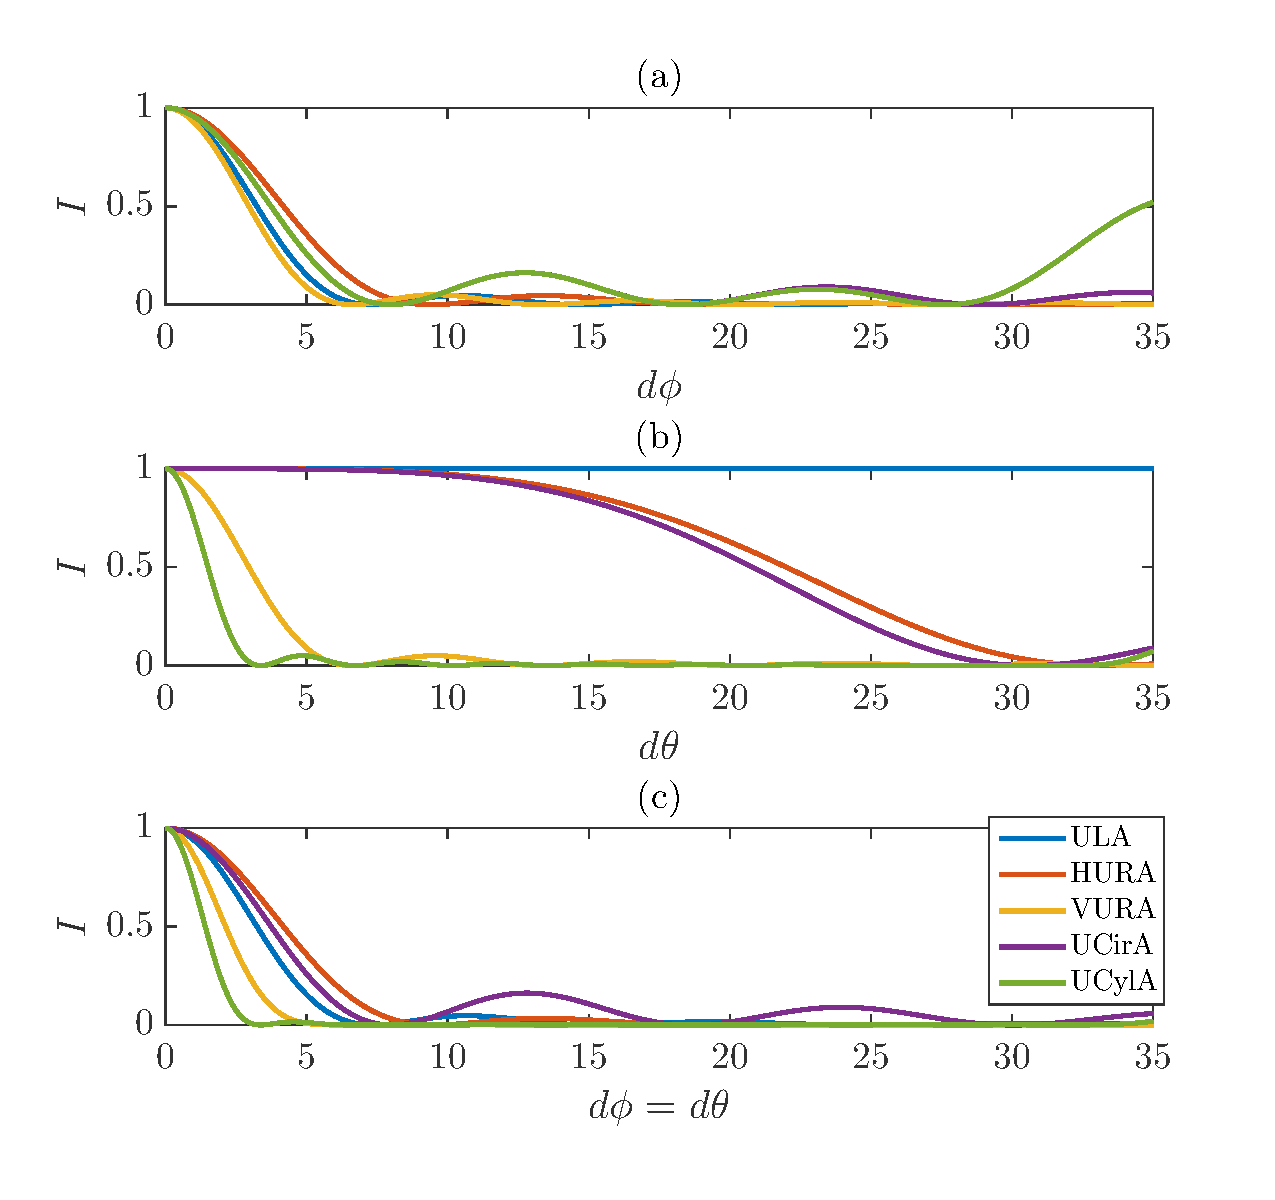
\includegraphics[width=1\columnwidth]{sample_figure.pdf}
	\caption{Here is a pdf figure incorporated in the document.}
	\label{fig:example}
\end{figure}

 \section{Conclusions}\label{Conc}


\end{document}